%!TEX root = ../main.tex

\chapter{Bayesian blocks}%
\label{apdx:bayesblocks}

The Bayesian block representation is a non-parametric representation of data derived with
a Bayesian statistical procedure. The idea has been introduced by Jeffrey D.~Scargle and
applied in the context of astronomical time series analysis~\cite{Scargle1997,
Scargle2012}. As a generic (non-parametric) way to present data, the algorithm can be
efficiently employed to discover local structures in background data by exploiting the
full information brought in by the data itself and imposing few preconditions as possible
on signal and background shapes. As it will be shown later, the algorithm is also able to
handle arbitrary sampling and dynamic ranges of data. But perhaps the most appealing
characteristic of the algorithm is that it operates in a Bayesian framework and therefore
works with posterior probabilities.

\blocktitle{algorithm}
The purpose of the Bayesian blocks algorithm is to construct a segmentation of a certain
data interval into variable-sized blocks, each block containing consecutive data elements
satisfying some well-defined criterion. Among all the possible segmentations, the
\emph{optimal} segmentation is defined as the one that maximizes some quantification of
this criterion. The latter is represented by a likelihood (or fitness) function, which
acts on a block $k$ and depends exclusively on the data contained by the block. The
fitness of the entire partition is then calculated as the product of each block fitness.
The chosen fitness function will then depend on a certain set of parameters, in
particular, the length spanned by the block (considering, for simplicity, one-dimensional
data). Once the fitness function is defined, the algorithm will marginalize it with
respect to all the other (nuisance) parameters, therefore obtaining the length of each
single block, or the final data segmentation.
\newpar
There is a considerable freedom in choosing the fitness function, relying on the concept
of \emph{sufficient statistics}. One of the simplest block model is perhaps the
\emph{piecewise constant model}, i.e.~a constant representation of data within a block. In
this example the fitness of a block depends on two parameters: the length and the height
(nuisance parameter) of the block. The Cash statistics can be then employed to build the
likelihood function. With a model $M(t, \theta)$ (the variable $t$ represents the data,
which is often time in applications of the Bayesian blocks), the unbinned log-likelihood
$\mathcal{L}$ reads:
\[
  \log \mathcal{L}(\theta) = \sum_n \log M(t_n, \theta) - \int M(t, \theta)dt
\]
which, considering the piecewise constant model $M(t, \lambda) = \lambda$, becomes for
block $k$:
\[
  \log \mathcal{L}^{(k)}(\lambda) = N^{(k)} \log\lambda - \lambda T^{(k)} \;.
\]
When maximizing the expression with respect to the nuisance parameter $\lambda$ (the
height of the block), it becomes
\[
  \log \mathcal{L}_\text{max}^{(k)} = N^{(k)}(\log N^{(k)} - \log T^{(k)}) + N^{(k)}
\]
The $N^{(k)}$ term sums up to $N$ so it can be dropped because it's independent of the
partition:
\[
  \log \mathcal{L}_\text{max}^{(k)} = N^{(k)}(\log N^{(k)} - \log T^{(k)}) + \cancel{N^{(k)}} \;.
\]
The obtained fitness function has the appealing properties of being relatively simple and
scale invariant. The fitness of the entire partition will then be the sum over the total
number of blocks:
\[
  \log \mathcal{L} = \sum_k \log L^{(k)}_\text{max}
\]

The next essential item in Bayesian statistics is the prior distribution, which must be
chosen for each model parameter, in this case the total number of blocks
$N_\text{blocks}$. A uniform prior on the number of blocks looks unreasonable, as most of
the times one looks for a data segmentation where $N_\text{blocks} \ll N$, the total
number of data points, rather than $N_\text{blocks} \approx N$. For example the
\emph{geometric} prior:
\[
  P(N_\text{blocks}) =
  \begin{cases}
    P_0\gamma^{N_\text{blocks}} & 0 \le N_\text{blocks} \le N \\
    0                           & \text{else}
  \end{cases}
\]
has well-understood properties ($\gamma < 1$) and is simply implemented in the algorithm.
The value of $\gamma$ affects the representation but note that, however, sharply defined
structures are retained. Objective procedures can be used to select the desired value of
$\gamma$, which express the trade-off between conservative and liberal positions in
letting faint data features emerge in the partition. In general, running the algorithm
with a few different values of $\gamma$ can be enough because the number of change-points
in the partition is generally insensitive to a large range of reasonable values of the
prior ``steepness'' parameter. This approach can be made rigorous by calibrating the prior
as a function of the number of data points $N$ and the false-positive (type-I error) rate
$p_0$ on pure-noise toy experiments, as suggested in~\cite{Scargle2012}. A calibration of
this type performed there yields:
\[
  \log P(N, p_0) = \log(73.53 p_0 N^{-0.478}) - 4 \;.
\]

\blocktitle{binning \\ histograms}
The Bayesian blocks algorithm was developed to be mainly applied to time series analyses
(e.g.~to spot light flux changes from astrophysical objects), but has advantages also in
binning histograms, as shown in~\cite{Pollack2017}. Compared to fixed-size bins, whose
width is often \emph{ad hoc}, Bayesian blocks surely are a more objective way to present
data and to reveal shape features that could be hid by certain fixed-width binnings. Using
Bayesian blocks to represent data in a statistical analysis could as instance avoid testing for
systematics effects arising from the choice of the bin size. Compared to other
optimal segmentation search rules (Knuth's rule, Scott's rule etc.), it has the feature of
using variable-width blocks, and is therefore attractive when representing not
homogeneously distributed data. An exhaustive comparison between this and similar
segmentation schemes is presented in~\cite{Pollack2017}. An example application of
Bayesian blocks to $Z_0$ boson resonance data is reported here in
\cref{fig:bayesblocks:dimuon}.
\begin{figure}
  \centering
  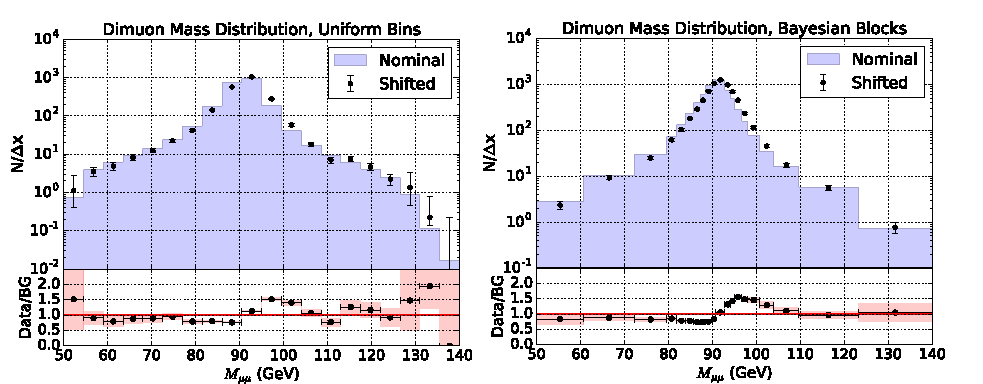
\includegraphics[width=0.9\linewidth]{plots/bblocks/dimuon-mass.pdf}
  \caption{
    Comparison of fixed-width binning and Bayesian blocks applied to the distribution of
    the invariant mass $M_{\mu\mu}$ of muon pairs produced at a hadron collider. A shift
    in the peak position between two data sets is clearly visible with Bayesian blocks.
    Taken from~\cite{Pollack2017}.
  }\label{fig:bayesblocks:dimuon}
\end{figure}

\blocktitle{implementation}
Sorting the optimality of $2^N$ data partitions is definitely not a quick task for a
computer, when $N$ is big. The central point of implementing an algorithm to compute
Bayesian blocks is to follow a \emph{dynamic programming} approach, in the spirit of
mathematical induction. In practice the data is first sorted in ascending order and the
algorithm, starting from the first point, updates the optimal data partition at each added
point using only the information from the previous steps. In this way, the algorithm
complexity is reduced from $\mathcal{O}(2^N)$ to $\mathcal{O}(N^2)$. A possible pseudo
code for the main iteration is the following:
\begin{lstlisting}[language=julia, style=jlcodestyle]
  for k in 1:N
      # define the (log) fitness function + (log) prior for a block
      # N(k,r) is the number of data points between point r and point k
      # T(k,r) is the distance between point r and point k
      F(r) = logfitness(N(k,r), T(k,r)) + log_prior
      # compute all possible configurations
      A = [F(r) + best[r-1] for r in 1:k]
      # save change-point with maximum fitness
      push!(last, indmax(A))
      # save maximum fitness value
      push!(best, maximum(A))
  end
\end{lstlisting}
What the algorithm does when adding a given data point \m{k} is to check whether a new
change-point should be added by considering a partition in which the last block contains
data points from \m{r} to \m{k}, where 0 < \m{r} < \m{k}. The total fitness is calculated
for all data points up to \m{k} by adding the fitness of the last block [\m{r}, \m{k}], to
the best fitness calculated at step \m{r}. The maximum is saved (\m{last}), along with the
fitness value (\m{best}). At the end of the iteration, the change-points can be
reconstructed from the \m{last} array.

\blocktitle{\gerda\ \\ data}
The \gerda\ data, which has a highly non-homogeneous event rate, benefits from being
represented with Bayesian blocks, rather than fixed-width bins which are used by default.
The results of the application of the algorithm to event energy data are displayed in
\cref{fig:bayesblocks:gerdadata}. Since the algorithm naturally assigns wider blocks to
less-populated regions, one can see how the binning is finer in the left part of the
spectrum, dominated by \Arl\ and \nnbb\ events, and it gets more coarse in the \a\
event-dominated region. Even finer binning is used for the high-statistics \kvn\ and \kvz\
lines. Bayesian blocks are also used to plot background model pdfs and calibration data,
see e.g.~\cref{fig:bkg:raw:ph2:pdfs:gmodel,fig:gerda:calib-desc}.

\begin{figure}
  \centering
  \includegraphics{plots/bblocks/gerda-data-merged-bblocks.pdf}
  \caption{%
    Histograms of \gerda\ data with Bayesian blocks. Histograms binned with 0.1~keV-wide
    bins are provided as input to the algorithm with the prior calibration parameter $p_0
    = 0.05$. In the three first rows, data after granularity cut. In the last row, data
    after LAr and PSD cut. \fillme{fill blinded region}
  }\label{fig:bayesblocks:gerdadata}
\end{figure}

\section*{Julia code}
The implementation of a routine that computes change points in an array of data applying
the Bayesian blocks algorithm is available in \m{C++} and Julia~\cite{Bezanson2017},
at the following link:
\begin{center}
  \url{https://github.com/gipert/bayesian-blocks}
\end{center}
The \m{C++} library ships with \m{bblocks}, a command line utility to re-bin
ROOT~\cite{Brun1997} histograms. The Julia code is reported also in the following.

% FIXME: this has to be loaded when using jlcode
\begin{lstlisting}[language=julia, style=jlcodestyle,
                   basicstyle={\loadcolors\small\ttfamily},
                   numbers=left,
                   stepnumber=1,
                   numberstyle={\color{jlcomment}\footnotesize\ttfamily}]
# bayesian_blocks.jl
#
# Author: Luigi Pertoldi - pertoldi@pd.infn.it
# Created: 29 Jun 2018
#
# The following software is distributed under the MIT licence
# http://www.opensource.org/licenses/mit-license.php
# Copyright (c) 2018 Luigi Pertoldi
#
# Use Julia >= v0.7!

using StatsBase, ProgressMeter

"""
    bayesian_blocks(data, logfitness=:cash, logprior=:p0, [gamma=0.01, p0=0.01])

Return an array of optimal change points for a set of one-dimensional data. This
is the implementation of the bayesian blocks algorithm, as outlined in [^1].

## Arguments
 * `data`: numeric array or a `StatsBase.Histogram`
 * `logfitness`: log of the block fitness function to be used, choose between
                 [:cash]
 * `logprior`: log of the prior distribution on the number of blocks to be used,
               choose between [:gamma, :p0]
 * `gamma`, `p0`...: set the parameter value for the specified prior distribution

## Example
```julia
using Distributions, StatsBase, Plots, LinearAlgebra

data = vcat(rand(Normal(0),1000),rand(Cauchy(5),1000))
data = data[(data .> -5) .& (data .< 10)]

h = fit(Histogram, gerda, -5:100:10, closed = :left)

# choose to use all data or an histogram of it!
hb = normalize(fit(Histogram, data, bayesian_blocks(data), closed = :left))
hb = normalize(fit(Histogram, data, bayesian_blocks(h),    closed = :left))

plot(data, st = :stephist, normalized = true, nbins=1000)
plot!(hb, st = :step, w = 3)
```

### Performance tips
You can convert your data container to a less precise representation to improve
the performance a bit, e.g.
```julia
x::Array{Float32} = [1.1, π, (√5-1)/2]
```

[^1]: Scargle, J et al. (2012) [https://arxiv.org/abs/1207.5578]
"""
function bayesian_blocks(x;
                         logfitness::Symbol=:cash, logprior::Symbol=:p0,
                         gamma=0.01, p0=0.01)

    if typeof(x) <: Array{<:Real,1}
        # take care of repeated data
        x_sorted = sort(x)
        x_unique = [x_sorted[1]]
        x_weight::Array{Int32} = [1]
        for i in 2:length(x_sorted)
            if x_sorted[i] == x_sorted[i-1]
                x_weight[end] += 1
            else
                push!(x_unique, x_sorted[i])
                push!(x_weight, 1)
            end
        end
    elseif typeof(x) <: Histogram{<:Integer,1}
        v = collect(x.edges[1])
        x_unique = [0.5 * (v[i] + v[i + 1]) for i = 1:length(v) - 1]
        x_weight = x.weights

        # delete empty bins
        deleteat!(x_unique, findall(iszero, x_weight))
        deleteat!(x_weight, findall(iszero, x_weight))
    else
        error("Unsupported input type: $(typeof(x))")
    end

    # final number of data points
    N = length(x_unique)

    # pre-defined (log)fitness functions
    logf_dict = Dict(
        :cash => (N_k, T_k) -> N_k * log(N_k/T_k)
    )

    # pre-defined (log)prior distributions on Nblocks
    logp_dict = Dict(
        # simple γ^Nblocks prior
        :gamma => (γ=gamma) -> log(γ),
        # Note that there is a mistake in this equation in the original Scargle
        # paper (the "log" was missing). The following corrected form is taken
        # from https://arxiv.org/abs/1304.2818
        :p0    => (Np=N, p=p0) -> log(73.53 * p * Np^(-0.478)) - 4
    )

    # check input
    !haskey(logf_dict, logfitness) && error("$logfitness function not defined!")
    !haskey(logp_dict, logprior)   && error("$logprior function not defined!")

    # save prior value for later computation
    ncp_prior = logp_dict[logprior]()

    # array of (all possible) block edges
    edges = vcat(x_unique[1],
                 0.5f0(x_unique[1:end-1]+x_unique[2:end]),
                 x_unique[end])

    # see Sec. 2.6 in [^1]
    best = Number[]
    last = Number[]

    # display progress bar for long computations
    # total number of steps: ∑n(n-1) = N(N^2-1)/3
    p = Progress(Integer(N*(N^2-1)/3), 2); m = 0

    for k in 1:N
        # define nice alias to mimic the notation used in [^1]
        F(r) = logf_dict[logfitness](cumsum(x_weight[r:k])[end], edges[k+1] - edges[r]) + ncp_prior

        # compute all possible configurations (Eq. (8) in [^1])
        A = [F(r) + (r == 1 ? 0 : best[r-1]) for r in 1:k]

        # save best configuration
        push!(last, argmax(A))
        push!(best, maximum(A))

        update!(p, m += k*(k-1))
    end

    # extract changepoints by iteratively peeling off the last block
    cp = Number[]
    i = N+1
    while i != 0
        push!(cp, i)
        i = (i == 1 ? 0 : last[i-1])
    end

    return [edges[j] for j in cp[end:-1:1]]
end
\end{lstlisting}

% vim: tw=90
